\pagebreak
\section{Appendix}

\subsection{Code}
I have placed the code used for the project at: https://github.com/sayedmcmaster/cas-764-food-group-acr-cluster/code %\footnote{My understanding is this subsection ideally belongs to appendix}. https://github.com/sayedmcmaster/cas-764-food-group-acr-cluster/codeoutput A list of the files and purpose is given below:

%\begin{figure}
%\begin{tabular}{|c|c|}
%\hline
%File & Purpose\\
%\hline
%$xpt\_to\_csv\_all\_files\_in\_a\_folder.ipynb$ & converts SAS XPT data files to CSV files. It converts demographics, ACR Lab Data, and Dietary Intake data into CSV files. It shows a drop-down to select the Input File and the Input data format file and then convert it. It could convert any other XPT data file such as Blood Pressure data files to CSV files as well. \\
%\hline
%\end{tabular}
%\caption{\textbf{GFR, ACR and Kidney Disease (Ref: Google Images)}}
%\label{gfr-acr-ckd-methodology}
%\vspace{0.25cm}
%\end{figure}


\subsection{Dataset Generation}
Initially, I wrote and used Python code ($xpt\_to\_csv\_all\_files\_in\_a\_folder.ipynb$) to generate data files for each year (Demographics, ACR, Dietary Intake). Then I brought the data into MS SQL Server. Then wrote and used Stored Procedures to combine each category of data, and then used another stored procedure (dietaryIntakeDataForClassificationAndAnalysis. StoredProcedure. sql) to join all these data to create the big dataset for analysis. The stored procedures can be found on GitHub under 'sayedmcmaster/cas-764-food-group-acr-cluster/code/SQL/storedprocedures/' and in Figure ~\ref{sp-combine}. This is what I used initially. However, later I wrote another Python code $automated\_xpt\_to\_csv\_all\_files.ipynb$ that can create CSV files from XPT one by one iteratively. This code ideally can combine all data input given in one shot provided the columns align. Also, wrote another Python code to merge one category of data files (I also have a stored procedure). Both approaches have some pros and cons. I am using and planning to use them as they seem appropriate. \footnote{Because the code and SQLs are only for my use, I am not making them perfect considering coding standards and performance}

\begin{figure}[!htb]
\begin{tabular}{c}
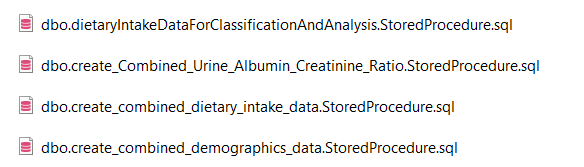
\includegraphics[scale=1]{images/datasetgenerationcode/create-data-set.png} \\
\end{tabular}
\caption{\textbf{Stored Procedures to Combine Data and to create big dataset}}
\label{sp-combine}
\vspace{0.25cm}
\end{figure}

\subsubsection{Code for Automated (semi-automated) CSV Data generation from XPT files}
File: $automated\_xpt\_to\_csv\_all\_files.ipynb$, Figure: ~\ref{automated-data-year}, ~\ref{automated-data-traverse}, ~\ref{automated-data-csv}

\begin{figure}[!htb]
\begin{tabular}{c}
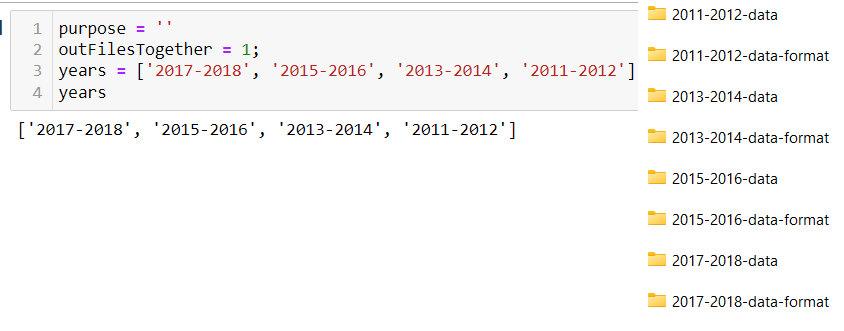
\includegraphics[scale=1]{images/datasetgenerationcode/set-years.png} \\
\end{tabular}
\caption{\textbf{Set all years to work on, Data Folder Structure}}
\label{automated-data-year}
\vspace{0.25cm}
\end{figure}

\begin{figure}[!htb]
\begin{tabular}{c}
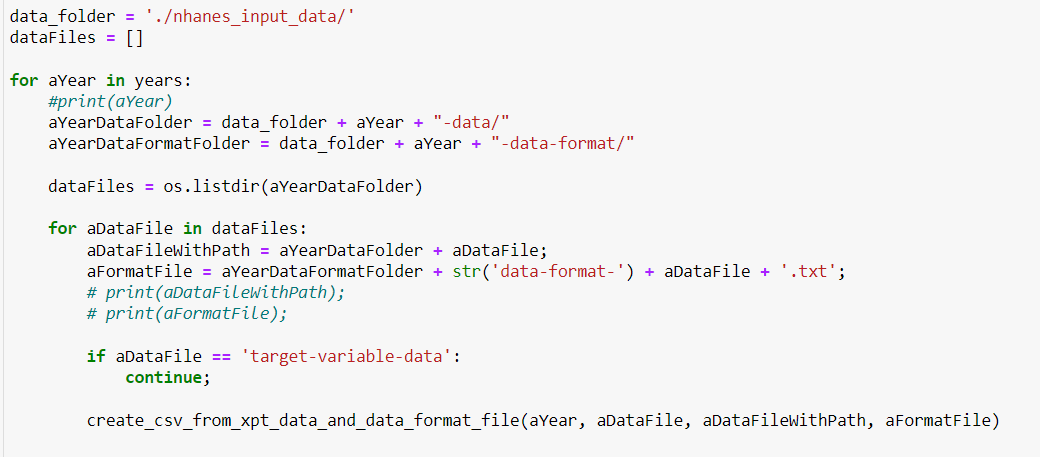
\includegraphics[scale=0.8]{images/datasetgenerationcode/convert-all-input-datafiles-for-multiple-years-into-csv-files.png} \\
\end{tabular}
\caption{\textbf{Traverse all data files and send them for conversion to CSV files}}
\label{automated-data-traverse}
\vspace{0.25cm}
\end{figure}


\begin{figure}[!htb]
\begin{tabular}{c}
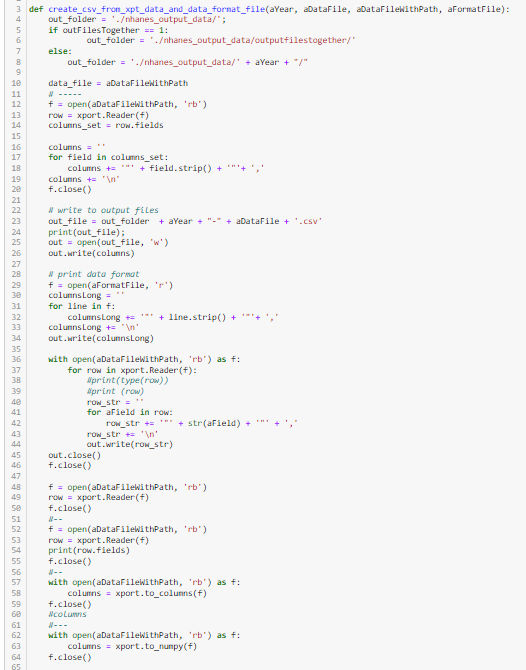
\includegraphics[scale=1]{images/datasetgenerationcode/code-writing-data-one-file-at-a-time.png} \\
\end{tabular}
\caption{\textbf{Code for Automated (semi-automated) Dataset Generation. create the CSV files with data}}
\label{automated-data-csv}
\vspace{0.25cm}
\end{figure}

%\pagebreak
\subsubsection{Merge Data Files from Multiple Years }
File: $merge-multiple-csv-files-with-python$, Figure: ~\ref{merge-data-files}, Purpose: We can configure this file to merge all demographics data or all dietary data, or all ACR data from multiple years into one. Some column alignments are needed in some cases where columns differ from year to year. I used Winmerge software to see the differences in data format.
\begin{figure}[!htb]
\begin{tabular}{c}
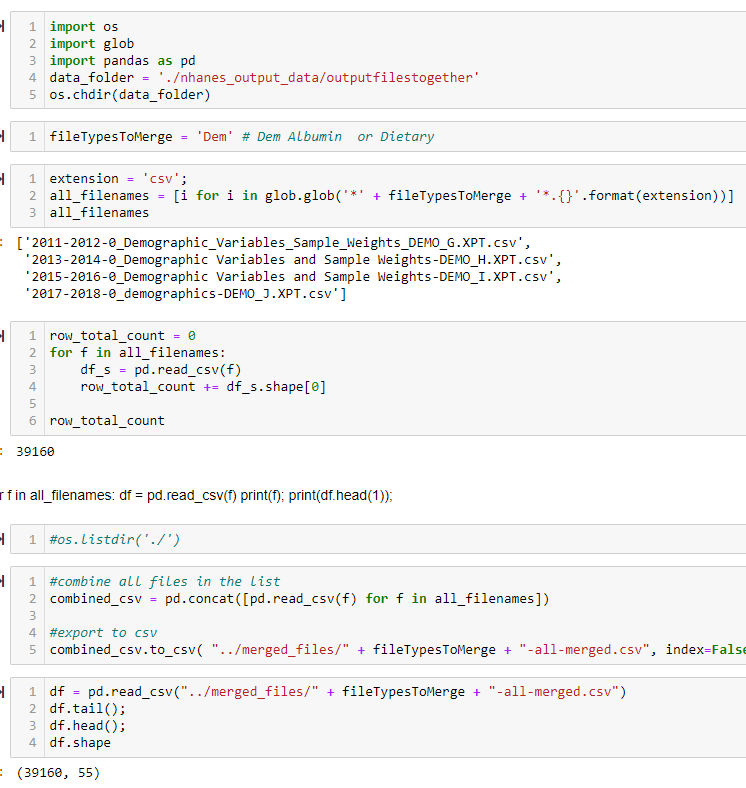
\includegraphics[scale=1]{images/datasetgenerationcode/merge-demographics-files.png} \\
\end{tabular}
\caption{\textbf{Merge Data Files from Multiple Years by category}}
\label{merge-data-files}
\vspace{0.25cm}
\end{figure}

%\pagebreak
\subsubsection {Cluster/Group Generation}
I have written a code in Python to create clusters as can be seen in Figure ~\ref{python-cluster}.
File: $cleaned-classifyDataBasedOnAgeAcrLevelAndThenTakeTheDietaryIntakeData.ipynb$ can be found on GitHub under the code folder. I also have written and used stored procedures to create clusters such as
$dbo.create\_a\_class\_group\_dataset.StoredProcedure.sql$ and $dbo.create\_classified\_dataset.StoredProcedure.sql$. These can be found in GitHub under code/SQL/storedprocedures/. I have used both Python and Stored Procedures to create clusters and verify that the output is correct \footnote{If data types in database tables are not correct for age, ACR then Python may not give correct clusters. Python code needs to use type casting}.

\begin{figure}[!htb]
\begin{tabular}{c}
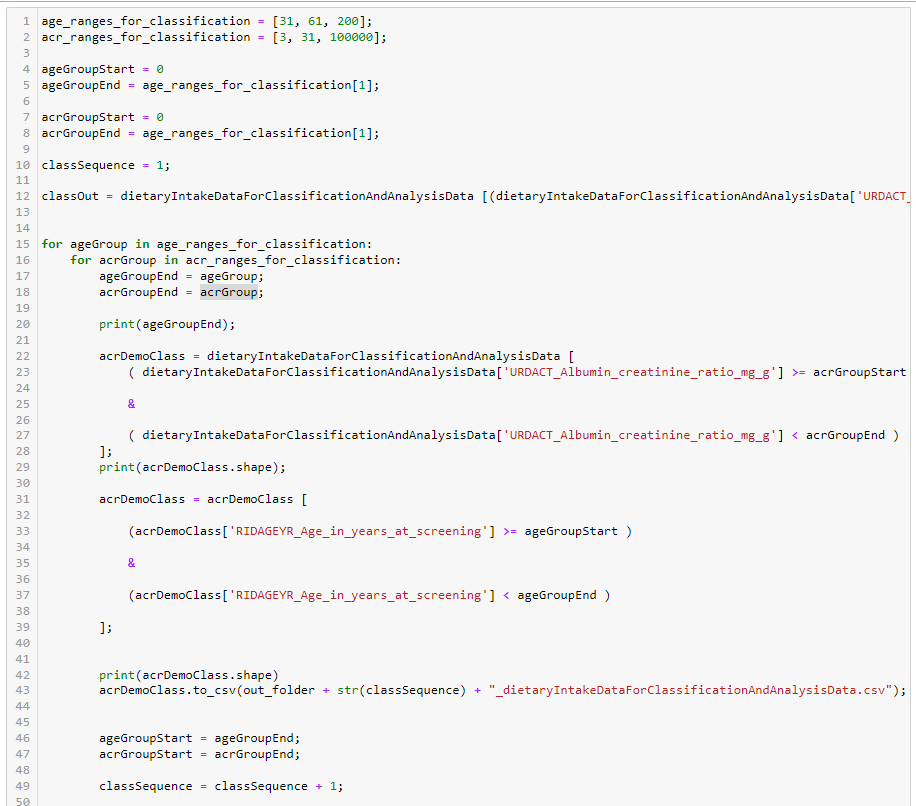
\includegraphics[scale=0.8]{images/datasetgenerationcode/cluster-python-code.png} \\
\end{tabular}
\caption{\textbf{Python Code to Create Clusters}}
\label{python-cluster}
\vspace{0.25cm}
\end{figure}


\subsection{Correlation of Food Groups with ACR}
Code File: $cleaned-foodgroup-acr-ratio-relation-by-agegroups-and-foods$. The code file can be found on GitHub under 'sayedmcmaster/cas-764-food-group-acr-cluster/tree/main/code/Exploratory Analysis/'. This code file generated the important food groups and correlation results as shown under the Results and Discussion section in figures ~\ref{pca-v-food-comp}, ~\ref{cluster-food-contribution}, ~\ref{corr-acr-food}, and ~\ref{corr-acr-food22}.

\subsection{Regression Coefficients contributing to ACR readings}
Code File: $regression-foodgroup-and-acr.ipynb$. The code file can be found on GitHub under: 'sayedmcmaster/cas-764-food-group-acr-cluster/tree/main/code'. This code file uses approaches such as Regression, Polynomial Regression, Random Forest, and Bayesian to find correlation coefficients of the food groups contributing to ACR readings. It finds correlations for the entire dataset as well as for the groups.

\subsection{K-Means Clustering}
I have implemented a proof of concept K-means algorithm to cluster the data. The data is clustered based on Age and ACR levels. However, if other data such as blood pressure is brought from NHANES, CDC then the clustering can also be updated with Age, ACR, and Blood Pressure. It just will need an update to the list of features to center around.
Code File: $kmeans-cleaned-and-code-combined-in-less-number-of-blocks$. The cluster data created with Kmeans can be found under $code/nhane_output_data/classifiedGroups/kmeanscluster$.
